\section{Horizontal tangent: \addbs{tkzTabTan} and \addbs{tkzTabTanFrom}}
\subsection{Definition of \tkzcname{tkzTabTan}}

\begin{NewMacroBox}{tkzTabTan}{\oarg{local options}\{Begin\}\{End\}\{Position\}\{Image\}}

\begin{tabular}{lllc}
\toprule
\texttt{arguments}   & \texttt{default}    & \texttt{definition}         \\
\midrule
\IargName{tkzTabTan}{Begin}&|no default|&rank of the start of the arrow   \\
\IargName{tkzTabTan}{End}&|no default|& rank of the end of the arrow   \\
\IargName{tkzTabTan}{Position}  & |no default|  & rank of the value of the variable     \\
\IargName{tkzTabTan}{Image}  & |no default|  & value of the image     \\
\bottomrule
\end{tabular}

\medskip
\noindent\emph{The first thing is to choose the arrow on which the tangent is placed. \tkzname{Begin} and \tkzname{End} are the ranks of the values at the ends of the arrow. \tkzname{Position} is the rank of the value where the tangent is. \tkzname{Image} is the value that can be written with the tangent (ordinate of the point of contact).}

\medskip
\begin{tabular}{lllc}
\toprule
\texttt{options}   & \texttt{default}    & \texttt{definition}                    \\
\midrule
\IoptName{tkzTabTan}{pos}     & |above| & position of the value                  \\
\bottomrule
\end{tabular}

\medskip
\noindent\emph{By default the value is placed above the tangent. The option \tkzname{pos} places it below: \tkzname{pos} alone means \tkzname{pos=below}.}

\end{NewMacroBox}


\subsection{Using the arguments}

\subsubsection{Plateau}
The arrow starts at the first value $0$, of rank $1$, and ends at $+\infty$, the value of rank $3$. Here the tangent is at $x=1$, the value of rank $2$.

\begin{tkzexample}[vbox]
\begin{tikzpicture}
 \tkzTab[espcl=6]{$x$/1,$f'(x)$ /1, $f$/3}%
 {$0$ , $1$ , $+\infty$}%
 {d , + , 0 , + , }
 {D- / $-\infty$ , R /  , +/ $+\infty$}%
 \tkzTabTan{1}{3}{2}{\scriptsize $2$}
\end{tikzpicture}
\end{tkzexample}

\subsubsection{Tangent at the end of an interval}
In the example below, the arrow starts at the first value $0$, of rank $1$, and ends at $1$, the value of rank $2$. Here the tangent is at $x=1$, the value of rank $2$. Note that the macro \tkzcname{tkzTabTan} applies to the line of variations just before it.

The image $0$ of $1$ by $f$ is not given in \tkzcname{tkzTabVar}: it would be under the arrows of the tangent. It is given as an argument of \tkzcname{tkzTabTan}, with the option \tkzname{pos=below}.

\begin{tkzexample}[vbox]
\begin{tikzpicture}
 \tkzTabInit[espcl=6]{$x$ /1,$f'(x)$/1,$f$/2}{$0$,$1$,$+\infty$}%
 \tkzTabLine{t , + , z , - , }%
 \tkzTabVar{-/ $-1$ , +/  , -/$-\infty$ }
 \tkzTabTan[pos=below]{1}{2}{2}{$0$}
\end{tikzpicture}
\end{tkzexample}

\subsection{Using the options}

\subsubsection{\texttt{\textcolor{red}{pos}}: position of the value}

\begin{tkzexample}[vbox]
\begin{tikzpicture}
 \tkzTabInit[espcl=5]{$x$/1,$f''{x}$/1,$f'(x)$/2,$f(x)$/2}{$0$,$1$,$+\infty$}%
 \tkzTabLine{d,+,0,-,}%
 \tkzTabVar{-/ $-\infty$  ,+/ ,-/$-\infty$}
 \tkzTabTan[pos=below]{1}{2}{2}{$0$}
 \tkzTabVar{+/ $+\infty$ , R/ , -/ $0$}
 \tkzTabTan{1}{3}{2}{$1$}
\end{tikzpicture}
\end{tkzexample}

\subsubsection{Nested variations}
\begin{tkzexample}[vbox]
\begin{tikzpicture}
  \tkzTabInit[espcl=3]
  {$x$      /1,
   $f''(x)$ /1,
    $f'$    /3,
     $f$    /3}%
  {$0$ , $\alpha$ , $1$ , $\beta$, $+\infty$ }%
  \tkzTabLine {d , +,  , + , z , - , , - }%
  \tkzTabVar {-/ $-1$  / , R/ ,+/ , R/ , -/ $-\infty$ }
  \tkzTabIma[draw]{1}{3}{2}{0}
  \tkzTabIma[draw]{3}{5}{4}{0}
  \tkzTabTan[pos]{1}{3}{3}{$2$}
  \tkzTabVar{+/ $+\infty$ , - / , R/,+/  , -/ $0$ }
  \tkzTabTan[]{1}{2}{2}{$1$}
  \tkzTabTan[pos=below]{2}{4}{4}{$2$}
\end{tikzpicture}
\end{tkzexample}


\subsection{Definition of \textcolor{red}{tkzTabTanFrom}}

\begin{NewMacroBox}{tkzTabTanFrom}{\oarg{local options}\{Begin\}\{End\}\{Position\}\{Image\}}

\begin{tabular}{lllc}
\toprule
\texttt{arguments}   & \texttt{default}    & \texttt{definition}         \\
\midrule
\IargName{tkzTabTanFrom}{Begin} & |no default|  & rank of the start of the arrow       \\
\IargName{tkzTabTanFrom}{End} & |no default|  & rank of the end of the arrow     \\
\IargName{tkzTabTanFrom}{Position} & |no default|  & name of a point        \\
\IargName{tkzTabTanFrom}{Image} & |no default|  & value of the image        \\
\bottomrule
\end{tabular}

\medskip
\noindent\emph{The position is given by the name of a point or of a node.}

\medskip
\begin{tabular}{lllc}
\toprule
\texttt{options}   & \texttt{default}    & \texttt{definition}       \\
\midrule
\IoptName{tkzTabTan}{pos}     & |above| & position of the value      \\
\bottomrule
\end{tabular}


\end{NewMacroBox}
\subsection{The name is defined by the table}
Here the name of the node that corresponds to $\alpha$ is \tkzname{N21} (value of rank 2, first rule below the value).
\begin{tkzexample}[vbox,small]
\begin{tikzpicture}
\tkzTabInit[ espcl=6]
{ $x$              /1,
  $f'(x)$          /1,
  $f$              /3}
{ $0$ ,  $\alpha$ , $+\infty$ }%
\tkzTabLine { , ,+, , }%
\tkzTabVar{-/ $-1$ , R , +/ $+1$ /}%
\tkzTabTanFrom[pos=below]{1}{3}{N21}{$0$}
\end{tikzpicture}
\end{tkzexample}

\subsection{The name is given by the user with the option \texttt{\textcolor{red}{remember}}}

\begin{tkzexample}[vbox,small]
\begin{tikzpicture}
\tkzTabInit[ espcl=4]
{ $x$              /1,
  $f''(x)$         /1,
  $f'$          /2,
  Sign of $f'(x)$ /2,
  $f$           /3}
{ $0$ , $1$ , $\alpha$ , $+\infty$ }%
\tkzTabLine {d,+,0,-, ,- }%
\tkzTabVar
{-/ $1$       ,
 +/           ,
 R/           ,
 -/ $-\infty$ }%
\tkzTabTan[pos,remember=v1]{1}{2}{2}{$2$}%
\tkzTabVal[remember=v2]{2}{4}{0.5}{}{0}%
\tkzTabLine { ,, +,, z,- }%
\tkzTabVar
{-/ $-\infty$ ,
 R/           ,
 +/           ,
 -/ $0$       }
\tkzTabImaFrom[]{1}{3}{v1}{0}%
\tkzTabImaFrom[]{3}{4}{v2}{}%
\tkzTabTanFrom[pos=below]{3}{4}{v2}{$1$}
\end{tikzpicture}
\end{tkzexample}


\endinput